%-----------------------------------------------------------------------
% Usar opção handout para disponibilizar slides
\documentclass[handout,serif, professionalfont, usenames, dvipsnames, aspectratio = 169]{beamer}\usepackage[]{graphicx}\usepackage[]{color}
% maxwidth is the original width if it is less than linewidth
% otherwise use linewidth (to make sure the graphics do not exceed the margin)
\makeatletter
\def\maxwidth{ %
  \ifdim\Gin@nat@width>\linewidth
    \linewidth
  \else
    \Gin@nat@width
  \fi
}
\makeatother

\definecolor{fgcolor}{rgb}{0.396, 0.482, 0.514}
\newcommand{\hlnum}[1]{\textcolor[rgb]{0.863,0.196,0.184}{#1}}%
\newcommand{\hlstr}[1]{\textcolor[rgb]{0.863,0.196,0.184}{#1}}%
\newcommand{\hlcom}[1]{\textcolor[rgb]{0.576,0.631,0.631}{#1}}%
\newcommand{\hlopt}[1]{\textcolor[rgb]{0.345,0.431,0.459}{#1}}%
\newcommand{\hlstd}[1]{\textcolor[rgb]{0.396,0.482,0.514}{#1}}%
\newcommand{\hlkwa}[1]{\textcolor[rgb]{0.796,0.294,0.086}{#1}}%
\newcommand{\hlkwb}[1]{\textcolor[rgb]{0.522,0.6,0}{#1}}%
\newcommand{\hlkwc}[1]{\textcolor[rgb]{0.796,0.294,0.086}{#1}}%
\newcommand{\hlkwd}[1]{\textcolor[rgb]{0.345,0.431,0.459}{#1}}%
\let\hlipl\hlkwb

\usepackage{framed}
\makeatletter
\newenvironment{kframe}{%
 \def\at@end@of@kframe{}%
 \ifinner\ifhmode%
  \def\at@end@of@kframe{\end{minipage}}%
  \begin{minipage}{\columnwidth}%
 \fi\fi%
 \def\FrameCommand##1{\hskip\@totalleftmargin \hskip-\fboxsep
 \colorbox{shadecolor}{##1}\hskip-\fboxsep
     % There is no \\@totalrightmargin, so:
     \hskip-\linewidth \hskip-\@totalleftmargin \hskip\columnwidth}%
 \MakeFramed {\advance\hsize-\width
   \@totalleftmargin\z@ \linewidth\hsize
   \@setminipage}}%
 {\par\unskip\endMakeFramed%
 \at@end@of@kframe}
\makeatother

\definecolor{shadecolor}{rgb}{.97, .97, .97}
\definecolor{messagecolor}{rgb}{0, 0, 0}
\definecolor{warningcolor}{rgb}{1, 0, 1}
\definecolor{errorcolor}{rgb}{1, 0, 0}
\newenvironment{knitrout}{}{} % an empty environment to be redefined in TeX

\usepackage{alltt}
%\documentclass[serif, professionalfont, usenames, dvipsnames, aspectratio = 169]{beamer}
\usepackage[T1]{fontenc}

% \usetheme{Copenhagen}

% Definição do esquema de cores:
% 1. UFPR - Azul com cinza.
% 2. DEST - Roxo com cinza.
% 3. LEG - Laranjado com cinza.
\def\mycolorscheme{1}

% Caminho para a imagem de fundo com aspecto 16x9.
% \def\pathtobg{config/ufpr-fachada-baixo-1.jpg}
% \def\pathtobg{config/ufpr-fundo.jpg}
% \def\pathtobg{config/ufpr-fundo.jpg}
\def\pathtobg{config/ufpr-fundo-16x9.jpg}

% ATTENTION: preamble.tex contains all style definitions.
%-----------------------------------------------------------------------

% Palladio.
% \usepackage[sc]{mathpazo}
% \linespread{1.05}         % Palladio needs more leading (space between lines)
% \usepackage[T1]{fontenc}

% Kurier.
% \usepackage[light, condensed, math]{kurier}
% \usepackage[T1]{fontenc}

% Iwona.
% \usepackage[math, light, condensed]{iwona}

% \usepackage{cmbright}
% \usepackage[charter]{mathdesign}
% \usepackage{palatino}

% Roboto (with Iwona for maths).
% \usepackage[math]{iwona}
% \usepackage[sfdefault, light, condensed]{roboto}

% Source Sans Pro (with Iwona for maths).
% \usepackage[math]{iwona}
% \usepackage[default, light]{sourcesanspro}

% Lato (with Iwona for maths).
% \usepackage[math]{iwona}
% \usepackage[default]{lato}

% Fira Sans (with Iwona for maths).
\usepackage[math, light]{iwona}
\usepackage[sfdefault,light]{FiraSans} %% option 'sfdefault' activates Fira Sans as the default text font
\usepackage[T1]{fontenc}
\renewcommand*\oldstylenums[1]{{\firaoldstyle #1}}

% Font for code. ----------------------------
% \usepackage[scaled=.75]{beramono}
\usepackage{inconsolata}

\usepackage{amstext} % for \text macro
\usepackage{array}   % for \newcolumntype macro
\newcolumntype{L}{>{$}l<{$}} % math-mode version of "l" column type

% ATTENTION: needs complile with xelatex: `$ xelatex file.tex`
% \usepackage{fontspec}
% \setmonofont{M+ 1m}
% \setmonofont{M+ 1mn}
% \setmonofont{M+ 2m}

%-----------------------------------------------------------------------

% \usepackage{lmodern}
\usepackage{amssymb, amsmath}
\usepackage[makeroom]{cancel}
% \usepackage{ifxetex, ifluatex}
\usepackage{fixltx2e} % provides \textsubscript
\usepackage[utf8]{inputenc}
\usepackage[shorthands=off,main=brazil]{babel}
\usepackage{graphicx}
\usepackage{color}
\usepackage{xcolor}
\usepackage{setspace}
\usepackage{comment}
\usepackage{icomma}

%-----------------------------------------------------------------------
% Algumas configurações.

\setlength{\parindent}{0pt}
\setlength{\parskip}{6pt plus 2pt minus 1pt}
\setlength{\emergencystretch}{3em}  % prevent overfull lines
% \providecommand{\tightlist}{%
%   \setlength{\itemsep}{0pt}\setlength{\parskip}{0pt}}
\setcounter{secnumdepth}{0}

% Espaço vertical para o ambiente `quote`.
\let\oldquote\quote
\let\oldendquote\endquote
\renewenvironment{quote}{%
  \vspace{1em}\oldquote}{%
  \oldendquote\vspace{1em}}

%-----------------------------------------------------------------------
% Espaçamento entre items para itemize, enumerate e description.

% % itemize.
% \let\itemopen\itemize
% \let\itemclose\enditemize
% \renewenvironment{itemize}{%
%   \itemopen\addtolength{\itemsep}{0.25\baselineskip}}{\itemclose}
%
% % enumerate.
% \let\enumopen\enumerate
% \let\enumclose\endenumerate
% \renewenvironment{enumerate}{%
%   \enumopen\addtolength{\itemsep}{0.25\baselineskip}}{\enumclose}
%
% % description.
% \let\descopen\description
% \let\descclose\enddescription
% \renewenvironment{description}{%
%   \descopen\addtolength{\itemsep}{0.25\baselineskip}}{\descclose}

%-----------------------------------------------------------------------

% \usepackage[hang]{caption}
\usepackage{caption}
\captionsetup{font=footnotesize,
  labelfont={color=mycolor1, footnotesize},
  labelsep=period}

% \providecommand{\tightlist}{%
%   \setlength{\itemsep}{0pt}\setlength{\parskip}{0pt}}

%-----------------------------------------------------------------------

\usepackage{tikz}

% \def\pathtobg{/home/walmes/Projects/templates/COMMON/ufpr-fundo.jpg}
% \def\pathtobg{/home/walmes/Projects/templates/COMMON/ufpr-fundo-16x9.jpg}
% \def\pathtobg{/home/walmes/Projects/templates/COMMON/ufpr-fachada-dir-1.jpg}
% \def\pathtobg{/home/walmes/Projects/templates/COMMON/ufpr-fachada-esq-1.jpg}
% \def\pathtobg{/home/walmes/Projects/templates/COMMON/ufpr-perto-1.jpg}
% \def\pathtobg{/home/walmes/Projects/templates/COMMON/ufpr-fachada-baixo-1.jpg}

\ifx\pathtobg\undefined
\else
  \usebackgroundtemplate{
    \tikz[overlay, remember picture]
    \node[% opacity=0.3,
          at=(current page.south east),
          anchor=south east,
          inner sep=0pt] {
            \includegraphics[height=\paperheight, width=\paperwidth]{\pathtobg}};
  }
\fi

%-----------------------------------------------------------------------
% Definições de esquema de cores.

\ifx\mycolorscheme\undefined
  % UFPR.
  % http://www.color-hex.com/color-palette/2018
  \definecolor{mycolor1}{HTML}{015c93} % Título.
  \definecolor{mycolor2}{HTML}{363435} % Texto.
  \definecolor{mycolor3}{HTML}{015c93} % Estrutura.
  \definecolor{mycolor4}{HTML}{015c93} % Links.
  \definecolor{mycolor5}{HTML}{CECAC5} % Preenchimentos.
\else
  \if\mycolorscheme1
    % UFPR.
    \definecolor{mycolor1}{HTML}{015c93} % Título.
    \definecolor{mycolor2}{HTML}{363435} % Texto.
    \definecolor{mycolor3}{HTML}{015c93} % Estrutura.
    \definecolor{mycolor4}{HTML}{015c93} % Links.
    \definecolor{mycolor5}{HTML}{CECAC5} % Preenchimentos.
  \fi
  \if\mycolorscheme2
    % DEST.
    \definecolor{mycolor1}{HTML}{2a0e72} % Título.
    \definecolor{mycolor2}{HTML}{202E35} % Texto.
    \definecolor{mycolor3}{HTML}{2a0e72} % Estrutura.
    % \definecolor{mycolor3}{HTML}{8072a3} % Estrutura.
    \definecolor{mycolor4}{HTML}{2a0e72} % Links.
    % \definecolor{mycolor4}{HTML}{bfb9d1} % Links.
    % \definecolor{mycolor5}{HTML}{AEA79F} % Preenchimentos.
    \definecolor{mycolor5}{HTML}{CECAC5} % Preenchimentos.
  \fi
  \if\mycolorscheme3
    % LEG.
    \definecolor{mycolor2}{HTML}{363435} % Texto.
    % \definecolor{mycolor1}{HTML}{ff8000} % Título.
    % \definecolor{mycolor3}{HTML}{ff8000} % Estrutura.
    % \definecolor{mycolor4}{HTML}{ff8000} % Links.
    % \definecolor{mycolor1}{HTML}{E57300} % Título.
    % \definecolor{mycolor3}{HTML}{E57300} % Estrutura.
    % \definecolor{mycolor4}{HTML}{E57300} % Links.
    \definecolor{mycolor1}{HTML}{F67014} % Título.
    \definecolor{mycolor3}{HTML}{F67014} % Estrutura.
    \definecolor{mycolor4}{HTML}{F67014} % Links.
    % \definecolor{mycolor1}{HTML}{FE5C23} % Título.
    % \definecolor{mycolor3}{HTML}{FE5C23} % Estrutura.
    % \definecolor{mycolor4}{HTML}{FE5C23} % Links.
    \definecolor{mycolor5}{HTML}{222222} % Preenchimentos.
    \definecolor{mycolor5}{HTML}{383838} % Preenchimentos.
  \fi
\fi

\hypersetup{
  colorlinks=true,
  linkcolor=mycolor4,
  urlcolor=mycolor1,
  citecolor=mycolor1
}

%-----------------------------------------------------------------------
% ATTENTION: http://www.cpt.univ-mrs.fr/~masson/latex/Beamer-appearance-cheat-sheet.pdf

\usetheme{Boadilla}
\usecolortheme{default}

% \setbeamersize{text margin left=7mm, text margin right=7mm}
% \setbeamertemplate{frametitle}[default][left, leftskip=3mm]
% \addtobeamertemplate{frametitle}{\vspace{0.5em}}{}

\setbeamertemplate{caption}[numbered]
\setbeamertemplate{section in toc}[sections numbered]
\setbeamertemplate{subsection in toc}[subsections numbered]
\setbeamertemplate{sections/subsections in toc}[ball]{}
\setbeamertemplate{sections in toc}[ball]
\setbeamercolor{section number projected}{bg=mycolor1, fg=white}
\setbeamertemplate{blocks}[rounded]
\setbeamertemplate{navigation symbols}{}
\setbeamertemplate{frametitle continuation}{\gdef\beamer@frametitle{}}
% \setbeamertemplate{frametitle}[default][center]
% \setbeamertemplate{footline}[frame number]

\setbeamertemplate{enumerate items}[default]
\setbeamertemplate{itemize items}{\scriptsize\raise1.25pt\hbox{\donotcoloroutermaths$\blacktriangleright$}}

% Blocos.
% \addtobeamertemplate{block begin}{\vskip -\bigskipamount}{}
% \addtobeamertemplate{block end}{}{\vskip -\bigskipamount}
\addtobeamertemplate{block begin}{\vspace{0.5em}}{}
\addtobeamertemplate{block end}{}{\vspace{0.5em}}


% Rodapé.
\setbeamercolor{title in head/foot}{parent=subsection in head/foot}
\setbeamercolor{author in head/foot}{bg=mycolor4, fg=white}
\setbeamercolor{date in head/foot}{parent=subsection in head/foot, fg=mycolor3}

% Cabeçalho.
\setbeamercolor{section in head/foot}{bg=mycolor2, fg=mycolor4}
\setbeamercolor{subsection in head/foot}{bg=mycolor2, fg=white}

\setbeamercolor{title}{fg=mycolor1}       % Título dos slides.
\setbeamercolor{titlelike}{fg=title}
\setbeamercolor{subtitle}{fg=mycolor2}    % Subtítulo.
\setbeamercolor{institute in head/foot}{parent=palette primary} % Instituição.
\setbeamercolor{frametitle}{fg=mycolor1}  % De quadro.
\setbeamercolor{structure}{fg=mycolor3}   % Listas e rodapé.
\setbeamercolor{item projected}{bg=mycolor2}
\setbeamercolor{block title}{bg=mycolor5, fg=mycolor2}
\setbeamercolor{normal text}{fg=mycolor2} % Texto.
\setbeamercolor{caption name}{fg=normal text.fg}
% \setbeamercolor{footlinecolor}{fg=mycolor2, bg=mycolor5}
% \setbeamercolor{section in head/foot}{fg=mycolor2, bg=mycolor5}
\setbeamercolor{author in head/foot}{fg=white, bg=mycolor1}
\setbeamercolor{section in foot}{fg=mycolor4, bg=mycolor5}
\setbeamercolor{date in foot}{fg=mycolor4, bg=mycolor5}
\setbeamercolor{block title}{fg=white, bg=mycolor1}
\setbeamercolor{block body}{fg=black, bg=white!80!gray}
\setbeamercolor{block body}{fg=black, bg=white!80!gray}

% To remove empty brackets of \institution.
\makeatletter
\setbeamertemplate{footline}{
  \leavevmode%
  \hbox{%
    \begin{beamercolorbox}[
      wd=0.3\paperwidth, ht=2.25ex, dp=1ex, right]{author in head/foot}%
      \usebeamerfont{author in head/foot}\insertshortauthor{}\hspace*{1ex}
    \end{beamercolorbox}%
    \begin{beamercolorbox}[
      wd=0.6\paperwidth, ht=2.25ex, dp=1ex, left]{section in foot}%
      \usebeamerfont{title in head/foot}\hspace*{1ex}\insertshorttitle{}
      % \usebeamerfont{title in head/foot}\hspace*{1ex}\insertframetitle{}
    \end{beamercolorbox}%
    \begin{beamercolorbox}[
      wd=0.1\paperwidth, ht=2.25ex, dp=1ex, right]{date in foot}%
      \insertframenumber{}\hspace*{2ex}
    \end{beamercolorbox}
  }%
  \vskip0pt%
}
\makeatother

%-----------------------------------------------------------------------

% \usepackage{hyphenat}
\usepackage{changepage}

% Slide para o título das seções.
\AtBeginSection[]{
  \begin{frame}
    % \vfill
    \vspace{4cm}
    % \centering
    % \begin{beamercolorbox}[sep = 8pt, center, shadow = true, rounded = true]{title}
    \begin{beamercolorbox}{title}
      \begin{columns}
        \column{0.7\linewidth}
        {\LARGE\textbf \insertsectionhead}
      \end{columns}
    \end{beamercolorbox}
    \vfill
  \end{frame}
}

%-----------------------------------------------------------------------

%---- preamble-chunk-rnw.tex -------------------------------------------

% Knitr.

% ATTENTION: this needs `\usepackage{xcolor}'.
\definecolor{color_line}{HTML}{333333}
\definecolor{color_back}{HTML}{DDDDDD}

% Tamanho de fonte e distância entre linhas.
% \renewenvironment{knitrout}{
%   \renewcommand{\baselinestretch}{0.75}%\tiny
% }{}

% Tamanho de fonte e distância entre linhas.
\renewenvironment{knitrout}{%
 \setlength{\topsep}{-0.25ex}
 \renewcommand{\baselinestretch}{0.65}
 \footnotesize
}{}

% R output e todo `verbatim'.
\makeatletter
% \def\verbatim@font{\linespread{0.9}\textit\normalfont\ttfamily\footnotesize}
\def\verbatim@font{\linespread{0.9}\ttfamily\footnotesize}
\makeatother

% Cor de fundo e margens do `verbatim'.
\let\oldv\verbatim
\let\oldendv\endverbatim

\def\verbatim{%
  \par\setbox0\vbox\bgroup % Abre grupo.
  \vspace{-5px}            % Reduz margem superior.
  \oldv                    % Chama abertura do verbatim.
}
\def\endverbatim{%
  \oldendv                 % Chama encerramento do verbatim.
  % \vspace{0cm}           % Controla margem inferior.
  \egroup\fboxsep10px      % Fecha grupo.
  \usebox0
  % \noindent{\colorbox{color_back}{\usebox0}}\par
}

%-----------------------------------------------------------------------

%---- preamble-commands.tex --------------------------------------------

% Para fazer texto em duas colunas.
\newcommand{\mytwocolumns}[4]{
  % #1: Line width fraction for the left column , e.g. 0.5.
  % #2: Line width fraction for the right column.
  % #3: Content for the left column.
  % #4: Content for the right column.
  \begin{columns}[c]
    \begin{column}{#1\linewidth} %----------- left.
      #3
    \end{column} %--------------------------- left.
    \begin{column}{#2\linewidth} %----------- right.
      #4
    \end{column} %--------------------------- right.
  \end{columns}
}

%-----------------------------------------------------------------------
% Para fazer duas colunas no Rmd.

% Center vertical align.
\def\beginAHalfColumn{\begin{minipage}{0.49\textwidth}}%
\def\beginAlmostHalfColumn{\begin{minipage}{0.45\textwidth}}%
\def\beginAQuarterColumn{\begin{minipage}{0.23\textwidth}}%
\def\beginThreeQuartersColumn{\begin{minipage}{0.72\textwidth}}%
\def\beginAThirdColumn{\begin{minipage}{0.31\textwidth}}%
\def\beginTwoThirdsColumn{\begin{minipage}{0.64\textwidth}}%
\def\endColumns{\end{minipage}}%

% Top vertical align.
\def\beginAHalfColumnT{\begin{minipage}[t]{0.49\textwidth}}%
\def\beginAlmostHalfColumnT{\begin{minipage}[t]{0.45\textwidth}}%
\def\beginAQuarterColumnT{\begin{minipage}[t]{0.23\textwidth}}%
\def\beginThreeQuartersColumnT{\begin{minipage}[t]{0.72\textwidth}}%
\def\beginAThirdColumnT{\begin{minipage}[t]{0.31\textwidth}}%
\def\beginTwoThirdsColumnT{\begin{minipage}[t]{0.64\textwidth}}%

%---------------------------------------------------------------------
% Ambientes para frases como e sem imagem.

\newcommand{\myquote}[3]{
  % #1: caminho para a imagem.
  % #2: a frase/quotation.
  % #3: o autor.
  \begin{center}
    \begin{minipage}[c]{0.19\linewidth}
      \begin{center}
        \includegraphics[height=2.5cm]{#1}
      \end{center}
    \end{minipage}
    \begin{minipage}[c]{0.7\linewidth}
      \begin{flushright}
        \textit{#2}
        \vspace{1ex}

        -- #3
      \end{flushright}
    \end{minipage}
  \end{center}
}

\newcommand{\myphrase}[2]{
  % #1: a frase/quotation.
  % #2: o autor.
  \begin{center}
    \begin{minipage}[c]{0.19\linewidth}
    \end{minipage}
    \begin{minipage}[c]{0.7\linewidth}
      \begin{flushright}
        \textit{#1}
        \vspace{1ex}

        -- #2
      \end{flushright}
    \end{minipage}
  \end{center}
}

%-----------------------------------------------------------------------
% Comandos para texto em destaque.

\newcommand{\red}[1]{\textcolor{red}{#1}}
\newcommand{\blue}[1]{\textcolor{blue}{#1}}
\newcommand{\yellow}[1]{\textcolor{yellow}{#1}}
\newcommand{\orange}[1]{\textcolor{orange}{#1}}
\newcommand{\cyan}[1]{\textcolor{cyan}{#1}}
\newcommand{\violet}[1]{\textcolor{violet}{#1}}
\newcommand{\pink}[1]{\textcolor{pink}{#1}}
\newcommand{\olive}[1]{\textcolor{olive}{#1}}
\newcommand{\magenta}[1]{\textcolor{magenta}{#1}}

% \newcommand{\hi}[1]{%
%   \textcolor{ubuntu_orange}{#1}\xspace
% }

\usepackage{xspace}

% URLs com letra miuda.
\newcommand{\myurl}[1]{%
  {\tiny \url{#1}}\xspace
}

% Botões.
\newcommand{\btn}[1]{%
  \beamergotobutton{#1}\xspace
}

% Texto grande centralizado.
\newcommand{\centertitle}[1]{%
  \begin{center}
    {\LARGE \bfseries \hi{#1}}
  \end{center}
}

%-----------------------------------------------------------------------

%---- preamble-author.tex ----------------------------------------------

%\author[Walmes Zeviani $\cdot$ UFPR]{%
%      \href{http://leg.ufpr.br/~walmes}{Prof.~Walmes Zeviani} \\
%      \href{mailto:walmes@ufpr.br}{\small\tt walmes@ufpr.br}
%}

%\institute[DEST/UFPR]{
%  {Laboratório de Estatística e Geoinformação}\\
%  {Departamento de Estatística}\\
%  {Universidade Federal do Paraná}}

\institute[]{
%  {\small LEG: Laboratório de Estatística e Geoinformação}\\
  {\scriptsize Programa de Pós-Graduação em Informática}\\
  {\scriptsize Data Science \& Big Data Research Group}\\
  {\scriptsize Universidade Federal do Paraná}
}

% Logo na capa.
\titlegraphic{
  \vspace{-1em}
  %
\includegraphics[height=1.2cm]{config/dest-texto-2.png}\hspace{2em}
  %
\includegraphics[height=1.2cm]{config/transversais1.png}\hspace{2em}
  %
\includegraphics[height=1.2cm]{config/ufpr-transparent-600px.png}
}

%-----------------------------------------------------------------------

%---- preamble-refs.tex ------------------------------------------------

% Bibliography.

% %\usepackage[style=authoryear]{biblatex}
% \usepackage[authordate, bibencoding=auto, strict, backend=biber, natbib]{biblatex-chicago}
%
% % Use:
% %   \cite{<ref>}
% %   \parencite{<ref>}
% %   \fullcite{<ref>}
% %   \footfullcite{<ref>}
%
% % ATTENTION
% % Compilation: pdflatex > biber > pdflatex > pdflatex.
%
% % Calls refs.bib at preamble with:
% \addbibresource{config/refs.bib}

% abntex2cite -------------------------------

\usepackage[
  alf,
  abnt-emphasize=bf,
  abnt-etal-list=2,
  abnt-and-type=&]{abntex2cite}
% Use:
%   \cite{<ref>}
%   \citeonline{<ref>}

% ATTENTION
% Compilation: pdflatex > bibtex > pdflatex > pdflatex.

% Calls refs.bib at last frame with:
% \bibliography{config.refs}

\let\oldbibliography\thebibliography
\renewcommand{\thebibliography}[1]{%
  \oldbibliography{#1}%
  \setlength{\itemsep}{1em}%
}

%--------------------------------------------



%-----------------------------------------------------------------------
%-----------------------------------------------------------------------
%-----------------------------------------------------------------------

\title[Qualificação TH · McGLM]{
  \LARGE \bf Testes de hipóteses em modelos multivariados\\ de covariância linear generalizada 
  %\vspace{1em}
}

\subtitle[Qualificação]{
  \large { Qualificação de Mestrado}
}

%\author[Prof. Paulo Justiniano $\cdot$ UFPR]{%
%      \href{http://leg.ufpr.br/~paulojus}{Prof.~Paulo Justiniano Ribeiro Jr} \\
%      \href{mailto:paulojus@ufpr.br}{\small\tt paulojus@ufpr.br}
%}

\author[Lineu Alberto $\cdot$ PPGInformatica UFPR]{%
      Lineu Alberto Cavazani de Freitas \\
      Prof.~Wagner Hugo Bonat \\
      Prof.~Marco Antônio Zanata Alves%\\
      %\href{mailto:paulojus@ufpr.br}{\small\tt paulojus@ufpr.br}
}

%\date[]{
%   \textcolor{lightgrey}{2018/1}
%}

%\date{17 de março de 2020}

\date{2021}

%-----------------------------------------------------------------------
%-----------------------------------------------------------------------
%-----------------------------------------------------------------------
\IfFileExists{upquote.sty}{\usepackage{upquote}}{}
\begin{document}

\begin{frame}[plain]
   \titlepage
\end{frame}

%-----------------------------------------------------------------------

\begin{frame}{Sumário}
\tableofcontents
\end{frame}

%-----------------------------------------------------------------------

\section{Introdução}

%-----------------------------------------------------------------------

\begin{frame}
  \frametitle{Ciência de dados}
  \begin{itemize}
    \itemsep 2ex
  
  \item A ciência de dados é vista como um campo de estudo de natureza interdisciplinar que incorpora conhecimento de grandes áreas como estatística, ciência da computação e matemática \cite{ley2018makes}. 
  
  \item Tem diversos campos de interesse.

  \item Os métodos estatísticos são de fundamental importância em grande parte das etapas da ciência de dados \cite{weihs2018data}.
  
  \item Neste sentido, os modelos de regressão tem papel importante.
  
  \end{itemize}
\end{frame}

%-----------------------------------------------------------------------

\begin{frame}
  \frametitle{Modelos de regressão}

  Para entender minimamente um modelo de regressão, é necessário compreender o
  conceito de \textbf{fenômeno aleatório}, \textbf{variável aleatória} e \textbf{distribuição de probabilidade}.

  \begin{itemize}
    \itemsep 2ex

  \item Um \textbf{fenômeno aleatório} é situação na qual diferentes observações podem fornecer diferentes desfechos. 
  
  \item \textbf{Variáveis aleatórias} associam um valor numérico a cada desfecho possível do fenômeno. Podem ser discretas ou contínuas.
  
  \item Existem probabilidades associadas aos valores de uma variável aleatória. Estas probabilidades podem ser descritas por funções:
  
  \begin{itemize}
    \item função de probabilidade, para variáveis aleatórias discretas.
    \item função densidade de probabilidade, para variáveis aleatórias contínuas.
  \end{itemize}

  \end{itemize}
\end{frame}

%-----------------------------------------------------------------------

\begin{frame}
  
  \frametitle{Modelos de regressão}

  \begin{itemize}
    \itemsep 2ex

  \item Modelos probabilísticos que buscam descrever as probabilidades de variáveis aleatórias, as chamadas \textbf{distribuições de probabilidade}.
  
  \item Em problemas práticos, podemos buscar uma distribuição de probabilidades que melhor descreva o fenômeno de interesse. 
  
  \item Estas distribuições são descritas por funções. 
  
  \item Estas funções possuem parâmetros que controlam aspectos da distribuição.
  
  \item Os parâmetros são quantidades desconhecidas estimadas através dos dados.
  
  \end{itemize}

\end{frame}

%-----------------------------------------------------------------------

\begin{frame}
  \frametitle{Modelos de regressão}

  \begin{itemize}
    \itemsep 2ex

  \item Na análise de regressão busca-se modelar os parâmetros das distribuições de probabilidade como uma função de outras variáveis.
  
  \item Isto é feito através da decomposição do parâmetro da distribuição em outros parâmetros, chamados de parâmetros de regressão. 
  
  \item Assim, o objetivo dos modelos de regressão consiste em obter uma equação que explique a relação entre as variáveis explicativas e o parâmetro de interesse da distribuição de probabilidades selecionada para modelar a variável aleatória. 
  
  \item Em geral, o parâmetro de interesse da distribuição de probabilidades modelado em função das variávis explicativas é a média. 
  
  \end{itemize}
\end{frame}

%-----------------------------------------------------------------------

\begin{frame}
  \frametitle{Modelos de regressão}

  \begin{itemize}
    \itemsep 2ex

  \item O processo de análise via modelo de regressão parte de um conjunto de dados.
  
  \item Pode-se usar um modelo para modelar a relação entre a média de uma variável aleatória e um conjunto de variáveis explicativas. 
  
  \item Assume-se que a variável aleatória segue uma distribuição de probabilidades e que o parâmetro de média desta distribuição pode ser descrito por uma combinação linear de parâmetros de regressão associados às variáveis explicativas. 
  
  \item A obtenção destes parâmetros estimados se dá na chamada etapa de ajuste do modelo.
  
  \item Fazendo uso da equação resultante do processo é possível estudar a importância das variáveis explicativas sobre a resposta e realizar predições da variável resposta com base nos valores observados das variáveis explicativas. 
  
  \end{itemize}
\end{frame}

%-----------------------------------------------------------------------

\begin{frame}
  \frametitle{Modelos de regressão}

  \begin{itemize}
    \itemsep 2ex

  \item Existem modelos uni e multivariados. 
  
  \item Nos modelos univariados há apenas uma variável resposta e temos interesse em avaliar o efeito das variáveis explicativas sobre essa única resposta.
  
  \item No caso dos modelos multivariados há mais de uma resposta e o interesse passa a ser avaliar o efeito dessas variáveis sobre todas as respostas. 
  
  \item Existem inúmeras classes de modelos de regressão, mencionaremos neste trabalho três importantes classes: 
  \begin{itemize}
  \item Modelos lineares.
  \item Modelos lineares generalizados.
  \item Modelos multivariados de covariância linear generalizada. 
\end{itemize}

  \end{itemize}
\end{frame}


%-----------------------------------------------------------------------

\begin{frame}
  \frametitle{Modelo linear normal}

  \begin{itemize}
    \itemsep 2ex

  \item No cenário univariado, durante muitos anos o modelo linear normal \cite{galton} teve papel de destaque.
  
  \item Muito usado principalmente por suas facilidades computacionais. 
  
  \item Um dos pressupostos do modelo linear normal é de que a variável resposta, condicional às variáveis explicativas, segue a distribuição normal. 
  
  \item Quando tal pressuposto não era atendido, uma alternativa, por muito tempo adotada, foi buscar uma transformação da variável resposta, tal como a família de transformações Box-Cox \cite{boxcox64}. 
  
  \end{itemize}
\end{frame}

%-----------------------------------------------------------------------

\begin{frame}
  \frametitle{Modelos lineares generalizados}

  \begin{itemize}
    \itemsep 2ex

  \item O avanço computacional permitiu a proposição de modelos mais complexos, que necessitavam de processos iterativos para estimação dos parâmetros \cite{paula}. 
  
  \item A proposta de maior renome foram os modelos lineares generalizados (GLM) \cite{Nelder72}. 
  
  \item Essa classe de modelos permitiu a flexibilização da distribuição da variável resposta de tal modo que esta pertença à família exponencial de distribuições. 

  \item Em meio aos casos especiais de distribuições possíveis nesta classe de modelos estão a Bernoulli, binomial, Poisson, normal, gama, normal inversa, entre outras.  
  
  \end{itemize}
\end{frame}

%-----------------------------------------------------------------------

\begin{frame}
  \frametitle{Modelos multivariados de covariância linear generalizada}

  \begin{itemize}
    \itemsep 2ex

  \item Há casos em que são coletadas mais de uma resposta por unidade experimental e há o interesse de modelá-las em função de um conjunto de variáveis explicativas. 
  
  \item Neste cenário surgem os modelos multivariados de covariância linear generalizada (McGLM) \cite{Bonat16}. 
  
  \item Esta classe pode ser vista com uma extensão multivariada dos GLMs que permite lidar com múltiplas respostas de diferentes naturezas e, de alguma forma, correlacionadas. 

  \item O McGLM é uma classe flexível ao ponto de ser possível chegar a extensões multivariadas para modelos de medidas repetidas, séries temporais, dados longitudinais, espaciais e espaço-temporais.
  
  \end{itemize}
\end{frame}

%-----------------------------------------------------------------------

\begin{frame}
  \frametitle{Testes de hipóteses}

  \begin{itemize}
    \itemsep 2ex

  \item Em regressão, um interesse comum é o de verificar se a retirada de determinada variável explicativa do modelo geraria uma perda no ajuste. 
  
  \item Isto é feito através dos chamados testes de hipóteses. 

  \item Testes de hipóteses são ferramentas estatísticas que auxiliam no processo de tomada de decisão sobre valores desconhecidos (parâmetros) estimados por meio de uma amostra (estimativas).
  
  \item Podemos atribuir a teoria, formalização e filosofia dos testes de hipótese a Neyman, Pearson e Fisher.
  
  \end{itemize}
\end{frame}

%-----------------------------------------------------------------------

\begin{frame}
  \frametitle{Testes de hipóteses}

No contexto de modelos de regressão, três testes de hipóteses são comuns, todos baseados na função de verossimilhança: 

\begin{itemize}
  \item O teste da razão de verossimilhanças \cite{trv}.
  \item O teste Wald \cite{wald}.
  \item O teste do multiplicador de lagrange, também conhecido como teste escore \cite{score1}, \cite{score2}, \cite{score3}.
\end{itemize}


\end{frame}

%-----------------------------------------------------------------------

\begin{frame}
  \frametitle{LRT, WT, LMT}

  \begin{itemize}
    \itemsep 2ex

  \item Os três testes podem ser usados para verificar se a retirada de determinada variável do modelo prejudica o ajuste. 
  
  \item No caso do teste de razão de verossimilhanças, dois modelos precisam ser ajustados. 

  \item Já o teste Wald e o escore necessitam de apenas um modelo. 

  \item Os testes são assintóticamente equivalentes. 

  \item Em amostras finitas estes testes podem apresentar resultados diferentes \cite{conflict}.

  \end{itemize}

\end{frame}

%-----------------------------------------------------------------------

\begin{frame}
  \frametitle{Técnicas baseadas em testes de hipóteses}

  \begin{itemize}
    \itemsep 2ex

  \item Existem técnicas como a análise de variância (ANOVA) \cite{anova_fisher}. 
  
  \item O objetivo da técnica é a avaliação do efeito de cada uma das variáveis explicativas sobre a resposta. 

  \item Isto é feito através da comparação via testes de hipóteses entre modelos com e sem cada uma das variáveis explicativas.

  \item Permite que seja possível avaliar se a retirada de cada uma das variáveis gera um modelo significativamente pior quando comparado ao modelo com a variável. 

  \item Para o caso multivariado extende-se a técnica para a análise de variância multivariada \cite{manova}, a MANOVA. 

  \end{itemize}

\end{frame}

%-----------------------------------------------------------------------

\begin{frame}
  \frametitle{Proposta}

  \begin{itemize}
    \itemsep 2ex

  \item Considerando os McGLMs, não há discussão a respeito da construção de testes de hipóteses.
  
  \item Nosso objetivo geral é o desenvolvimento de testes de hipóteses para os McGLMs.

  \item Buscamos propor uma adaptação do teste de Wald clássico utilizado em modelos lineares para os McGLMs. 

  \end{itemize}

\end{frame}

%-----------------------------------------------------------------------

\begin{frame}
  \frametitle{Proposta}

Nosso trabalho tem os seguintes objetivos específicos: 

  \begin{itemize}
    \itemsep 2ex

  \item Adaptar o teste Wald para realização de testes de hipóteses gerais sobre parâmetros de McGLMs. 
  
  \item Implementar funções para efetuar tais testes, bem como funções para efetuar ANOVAs e MANOVAs para os McGLMs. 

  \item Avaliar as propriedades e comportamento dos testes propostos com base em estudos de simulação.

  \item Avaliar o potencial de aplicação das metodologias discutidas com base na aplicação a conjuntos de dados reais.

  \end{itemize}

\end{frame}

%-----------------------------------------------------------------------

\section{Revisão de literatura}

%-----------------------------------------------------------------------

\begin{frame}
  \frametitle{Revisão de literatura}
  
  A revisão de literatura compreeende 2 temas:
  
  \begin{itemize}
    \itemsep 2ex
  \item Modelos multivariados de covariância linear generalizada. 
  \item Testes de hipóteses. 
  \end{itemize}
\end{frame}

%-----------------------------------------------------------------------

\subsection{Modelos Multivariados de Covariância Linear Generalizada}

%-----------------------------------------------------------------------

\begin{frame}
  \frametitle{Modelos multivariados de covariância linear generalizada}
  \begin{itemize}
    \itemsep 2ex
  
  \item Os GLM são uma forma de modelagem para lidar com apenas uma resposta para dados de diferentes naturezas.  
  
  \item É uma classe de modelos flexível e aplicável a diversos tipos de problema.  
  
  \item Apresenta três importantes restrições:
    \begin{itemize}
      \item A incapacidade de lidar com observações dependentes. 
      \item A incapacidade de lidar com múltiplas respostas simultaneamente.
      \item Leque reduzido de distribuições disponíveis. 
    \end{itemize}

  \item Com o objetivo de contornar estas restrições, foram propostos os chamados Modelos Multivariados de Covariância Linear Generalizada (McGLM).
  
  \item Vamos discutir os McGLM como uma extensão dos GLM. 
  
  \end{itemize}
\end{frame}

%-----------------------------------------------------------------------

\begin{frame}
  \frametitle{GLM}
  
  Considere:

\begin{itemize}
  \item $\boldsymbol{Y}$ um vetor $N \times 1$ de valores observados da variável resposta.
  
  \item $\boldsymbol{X}$ uma matriz de delineamento $N \times k$
  
  \item $\boldsymbol{\beta}$ um vetor de parâmetros de regressão $k \times 1$. 
\end{itemize}

\end{frame}

%-----------------------------------------------------------------------

\begin{frame}
  \frametitle{GLM}

um GLM pode ser descrito da forma

\begin{equation}
      \begin{aligned}
        \mathrm{E}(\boldsymbol{Y}) &=
         \boldsymbol{\mu} =
            g^{-1}(\boldsymbol{X} \boldsymbol{\beta}),
            \\
        \mathrm{Var}(\boldsymbol{Y}) &=
          \Sigma =
          \mathrm{V}\left(\boldsymbol{\mu}; p\right)^{1/2}\left(\tau_0\boldsymbol{I}\right)\mathrm{V}\left(\boldsymbol{\mu}; p\right)^{1/2},
      \end{aligned}
\end{equation}

Em que:

  \begin{itemize}
    \itemsep 2ex
  
  \item $g(.)$ é a função de ligação. 
  
  \item $\mathrm{V}\left(\boldsymbol{\mu}; p\right)$ é uma matriz diagonal em que as entradas principais são dadas pela função de variância aplicada ao vetor $\boldsymbol{\mu}$. 
  
  \item $p$ é o parâmetro de potência. 
  
  \item $\tau_0$ o parâmetro de dispersão. 
  
  \item $\boldsymbol{I}$ é a matriz identidade de ordem $N\times N$.
  
  \end{itemize}
\end{frame}

%-----------------------------------------------------------------------

\begin{frame}

  \frametitle{GLM}
  
  \begin{enumerate}
  \item Função de variância potência. 
  
    \begin{itemize}
      \item caracteriza a família Tweedie de distribuições.
      \item função de variância é dada por $\vartheta\left(\boldsymbol{\mu}; p\right) = \mu^p$
      \item casos particulares: normal ($p$ = 0), Poisson ($p$ = 1), gama ($p$ = 2) e normal inversa ($p$ = 3). 
      \item \cite{Jorgensen87} e \cite{Jorgensen97}.
    \end{itemize}

  
  \item Função de dispersão Poisson–Tweedie.
  
    \begin{itemize}
      \item caracteriza a família Poisson-Tweedie de distribuições
      \item visa contornar a inflexibilidade da utilização da função de variância potência para respostas discretas. 
      \item função de dispersão dada por $\vartheta\left(\boldsymbol{\mu}; p\right) = \mu + \mu^p$
      \item casos particulares os mais famosos modelos para dados de contagem: Hermite ($p$ = 0), Neyman tipo A ($p$ = 1), binomial negativa ($p$ = 2) e Poisson–inversa gaussiana (p = $3$) 
      \item \cite{Jorgensen15}.
      
    \end{itemize}

  \item Função de variância binomial. 
  
    \begin{itemize}
      \item dada por $\vartheta(\boldsymbol{\mu}) = \mu(1 - \mu)$
      \item utilizada quando a variável resposta é binária, restrita a um intervalo ou quando tem-se o número de sucessos em um número de tentativas.
    \end{itemize}

\end{enumerate}

\end{frame}

%-----------------------------------------------------------------------

\begin{frame}
  \frametitle{cGLM}
  \begin{itemize}
    \itemsep 2ex
  
  \item Alternativa para problemas em que a suposição de independência entre as observações não é atendida. 
  
  \item A solução proposta é substituir a matriz identidade $\boldsymbol{I}$ da equação que descreve a matriz de variância e covariância por uma matriz não diagonal $\boldsymbol{\Omega({\tau})}$. 
  
  \item A matriz $\boldsymbol{\Omega({\tau})}$ é descrita como uma combinação de matrizes conhecidas \cite{Anderson73} \cite{Pourahmadi00}.
  
  \end{itemize}
\end{frame}

%-----------------------------------------------------------------------

\begin{frame}
  \frametitle{cGLM}
  
  A matriz $\boldsymbol{\Omega({\tau})}$ pode ser escrita como:

\begin{equation}
h\left \{ \boldsymbol{\Omega}(\boldsymbol{\tau}) \right \} = \tau_0Z_0 + \ldots + \tau_DZ_D,
\end{equation}

em que 
  
  \begin{itemize}
    \itemsep 2ex
    
  \item $h(.)$ é a função de ligação de covariância. 
  
  \item $Z_d$ com $d$ = 0,$\ldots$, D são matrizes que representam a estrutura de covariância presente nos dados. 
  
  \item $\boldsymbol{\tau}$ = $(\tau_0, \ldots, \tau_D)$ é um vetor $(D + 1) \times 1$ de parâmetros de dispersão. 
  
  \item Tal estrutura pode ser vista como um análogo ao preditor linear para a média e foi nomeado como preditor linear matricial. 
  
  \end{itemize}

\end{frame}

%-----------------------------------------------------------------------

\begin{frame}
  \frametitle{McGLM}
  \begin{itemize}
    \itemsep 2ex
  
  \item Pode ser entendido como uma extensão multivariada do cGLM. 
  
  \item Contorna as principais restrições presentes nos GLM. 

  \end{itemize}
  
  Considere
  
  \begin{itemize}
  \item $\boldsymbol{Y}_{N \times R} = \left \{ \boldsymbol{Y}_1, \dots, \boldsymbol{Y}_R \right \}$ uma matriz de variáveis resposta
  
  \item $\boldsymbol{M}_{N \times R} = \left \{ \boldsymbol{\mu}_1, \dots, \boldsymbol{\mu}_R \right \}$ uma matriz de valores esperados.
  
  \item $\Sigma_b$, uma martiz de ordem $R \times R$, que descreve a correlação entre as variáveis resposta
  
\end{itemize}

  Cada uma das variáveis resposta tem sua própria matriz de variância e covariância, responsável por modelar a covariância dentro de cada resposta, sendo expressa por

\begin{equation}
\Sigma_r =
\mathrm{V}_r\left(\boldsymbol{\mu}_r; p\right)^{1/2}\boldsymbol{\Omega}_r\left(\boldsymbol{\tau}\right)\mathrm{V}_r\left(\boldsymbol{\mu}_r; p\right)^{1/2}.
\end{equation}
  
\end{frame}

%-----------------------------------------------------------------------

\begin{frame}
  \frametitle{McGLM}
  
  Um MCGLM é descrito como

\begin{equation}
\label{eq:mcglm}
      \begin{aligned}
        \mathrm{E}(\boldsymbol{Y}) &=
          \boldsymbol{M} =
            \{g_1^{-1}(\boldsymbol{X}_1 \boldsymbol{\beta}_1),
            \ldots,
            g_R^{-1}(\boldsymbol{X}_R \boldsymbol{\beta}_R)\}
          \\
        \mathrm{Var}(\boldsymbol{Y}) &=
          \boldsymbol{C} =
            \boldsymbol{\Sigma}_R \overset{G} \otimes
            \boldsymbol{\Sigma}_b,
      \end{aligned}
\end{equation}

em que 
  
  \begin{itemize}
    
    \itemsep 0.5ex
    
  \item $\boldsymbol{\Sigma}_R \overset{G} \otimes \boldsymbol{\Sigma}_b = \mathrm{Bdiag}(\tilde{\boldsymbol{\Sigma}}_1, \ldots, \tilde{\boldsymbol{\Sigma}}_R) (\boldsymbol{\Sigma}_b \otimes \boldsymbol{I}) \mathrm{Bdiag}(\tilde{\boldsymbol{\Sigma}}_1^\top, \ldots, \tilde{\boldsymbol{\Sigma}}_R^\top)$ é o produto generalizado de Kronecker. 
  
  \item a matriz $\tilde{\boldsymbol{\Sigma}}_r$ denota a matriz triangular inferior da decomposição de Cholesky da matriz ${\boldsymbol{\Sigma}}_r$. 
  
  \item o operador $\mathrm{Bdiag}$ denota a matriz bloco-diagonal. 
  
  \item $\boldsymbol{I}$ uma matriz identidade $N \times N$.
  
  \item Toda metodologia do McGLM está implementada no pacote \emph{mcglm} \cite{mcglm} do software estatístico R.

  \end{itemize}
  
\end{frame}

%-----------------------------------------------------------------------

\begin{frame}[c, allowframebreaks]

\textbf{Funções de estimação}

As funções de estimação para os parâmetros de regressão (função quasi-score) e de dispersão (função de estimação de Pearson) são dadas por:

\begin{center}
$\psi_{\boldsymbol{\beta}}(\boldsymbol{\beta}, \boldsymbol{\lambda}) = \boldsymbol{D}^\top \boldsymbol{C}^{-1}(\mathcal{Y} - \mathcal{M})$

$\psi_{\boldsymbol{\lambda}_i}(\boldsymbol{\beta}, \boldsymbol{\lambda}) = \mathrm{tr}(W_{\boldsymbol{\lambda}i} (\boldsymbol{r}^\top\boldsymbol{r} - \boldsymbol{C})),  i = 1,.., Q$
\end{center}

Em que:

\begin{itemize}
  
  \item $\boldsymbol{\beta}_r$ denota um vetor $k_r \times 1$ de parâmetros de regressão.
  
  \item $\boldsymbol{\lambda}$ é um vetor $Q \times 1$ de parâmetros de dispersão.
  
  \item $\mathcal{Y}$ é um vetor $NR \times 1$ com os valores da matriz de variáveis respostas $Y_{N \times R}$ empilhados.
  
  \item $\mathcal{M}$ é um vetor $NR \times 1$ com os valores da matriz de valores esperados $M_{N \times R}$ empilhados.
  
  \item $\boldsymbol{D} = \nabla_{\boldsymbol{\beta}} \mathcal{M}$ 
é uma matriz $NR \times K$, e $\nabla_{\boldsymbol{\beta}}$ denota o 
operador gradiente.
  
  \item $W_{\boldsymbol{\lambda}i} = -\frac{\partial
    \boldsymbol{C}^{-1}}{\partial \boldsymbol{\lambda}_i}$ 
    
  \item $\boldsymbol{r} = (\mathcal{Y} - \mathcal{M})$
  
\end{itemize}

\end{frame}

% -----------------------------------------------------------------

\begin{frame}[c, allowframebreaks]

\textbf{Distribuição assintótica e algoritmo de estimação}

\begin{itemize}

  \item Para resolver o sistema de equações $\psi_{\boldsymbol{\beta}} = 0$ e $\psi_{\boldsymbol{\lambda}} = 0$ faz-se uso do algoritmo Chaser modificado:

$$
\begin{matrix}
\boldsymbol{\beta}^{(i+1)} = \boldsymbol{\beta}^{(i)}- S_{\boldsymbol{\beta}}^{-1} \psi \boldsymbol{\beta} (\boldsymbol{\beta}^{(i)}, \boldsymbol{\lambda}^{(i)}), \\ 
\boldsymbol{\lambda}^{(i+1)} = \boldsymbol{\lambda}^{(i)}\alpha S_{\boldsymbol{\lambda}}^{-1} \psi \boldsymbol{\lambda} (\boldsymbol{\beta}^{(i+1)}, \boldsymbol{\lambda}^{(i)}).
\end{matrix}
$$

  \item Seja $\boldsymbol{\hat{\theta}} = (\boldsymbol{\hat{\beta}^{\top}}, \boldsymbol{\hat{\lambda}^{\top}})^{\top}$ o estimador baseado em funções de estimação de $\boldsymbol{\theta}$.
  
  \item A distribuição assintótica de $\boldsymbol{\hat{\theta}}$ é:

$$
\boldsymbol{\hat{\theta}} \sim N(\boldsymbol{\theta}, J_{\boldsymbol{\theta}}^{-1}),
$$

\noindent $J_{\boldsymbol{\theta}}^{-1}$ é a inversa da matriz de informação de Godambe, dada por
  
$$J_{\boldsymbol{\theta}}^{-1} = S_{\boldsymbol{\theta}}^{-1} V_{\boldsymbol{\theta}} S_{\boldsymbol{\theta}}^{-\top},$$ 

\noindent em que $S_{\boldsymbol{\theta}}^{-\top} = (S_{\boldsymbol{\theta}}^{-1})^{\top}.$

\end{itemize}

\end{frame}

%-----------------------------------------------------------------------

\begin{frame}
  \frametitle{Exemplo tópicos}
  \begin{itemize}
    \itemsep 2ex
  \item item 1. 
  \item item 2. 
  \item item 3. 
  \item item 4. 
  \item item 5. 
  \item item 6. 
  \item item 7. 
  \item item 8. 
  \end{itemize}
\end{frame}

%-----------------------------------------------------------------------

\section{Slides modelo}

%-----------------------------------------------------------------------

\begin{frame}
  \frametitle{Exemplo tópicos}
  \begin{itemize}
    \itemsep 2ex
  \item item 1. 
  \item item 2. 
  \item item 3. 
  \item item 4. 
  \item item 5. 
  \item item 6. 
  \item item 7. 
  \item item 8. 
  \end{itemize}
\end{frame}

%-----------------------------------------------------------------------

\begin{frame}[plain]
  \frametitle{Slide sem rodapé}

\begin{itemize}
\item item 1.
\item item 2.
\item item 3.
\item item 4.
\end{itemize}

\end{frame}

%------------------------------------------------------------

\begin{frame}
  \frametitle{Slide com imagem na pasta pics}

\begin{figure}
    \centering
    
\includegraphics[width=.3\linewidth]{./pics/sapiens.jpeg}
    \caption{Harari, 2018}
\nocite{harari}
\end{figure}

\end{frame}

%--------------------------------------------------

\begin{frame}
  \frametitle{Slide com referencia}

\cite{diggle+chetwynd:2011}

\end{frame}

%--------------------------------------------------

\begin{frame}[fragile]
\frametitle{Slide com código R}

\begin{knitrout}
\definecolor{shadecolor}{rgb}{0.992, 0.965, 0.89}\color{fgcolor}\begin{figure}

{\centering 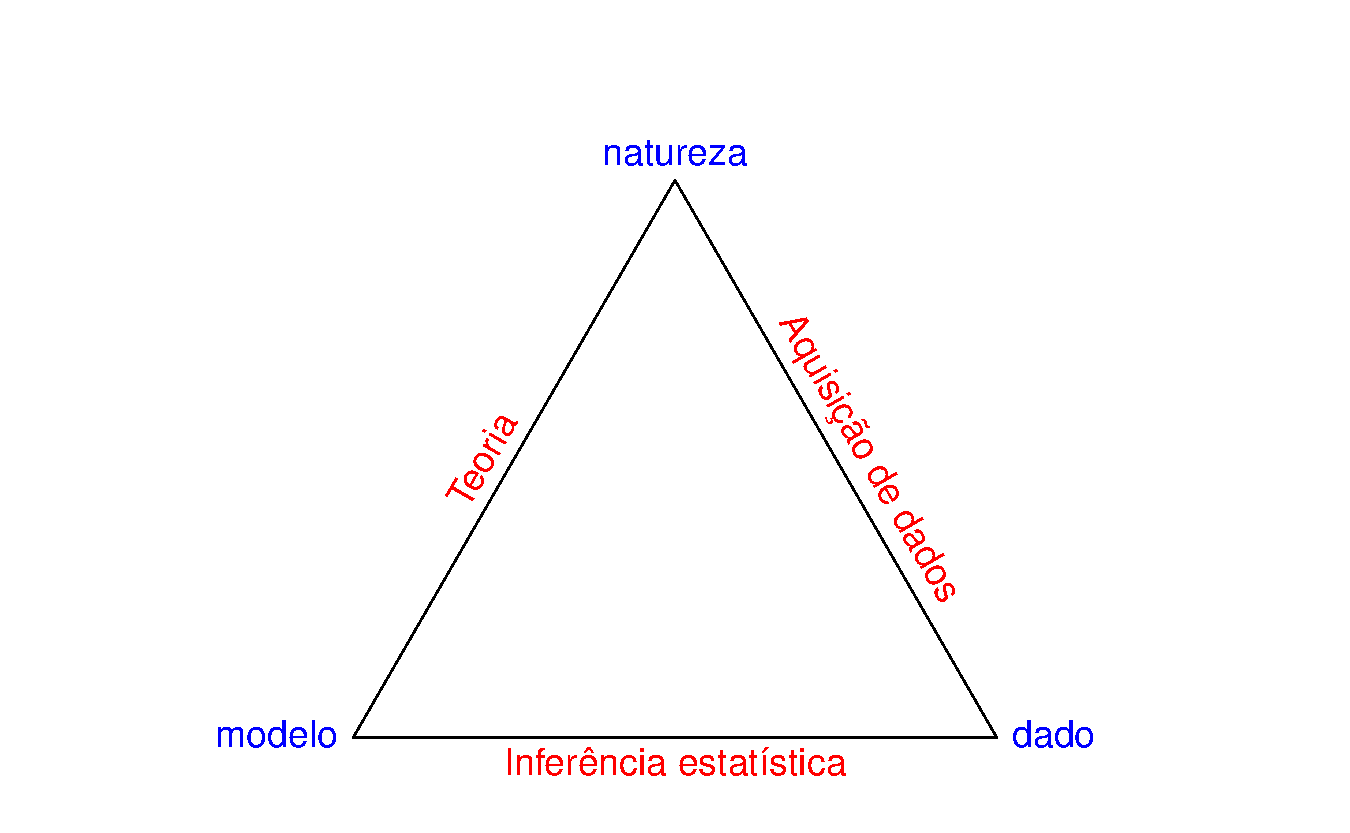
\includegraphics[width=11cm,height=0.75\textheight]{figure/unnamed-chunk-2-1} 

}

\caption{Estatística e o método científico (adaptado de \cite{diggle+chetwynd:2011}).}\label{fig:unnamed-chunk-2}
\end{figure}


\end{knitrout}
\end{frame}

%--------------------------------------------------

\begin{frame}[fragile]
  \frametitle{Referências bibliográficas}
  
  \begin{tiny}
    \bibliography{references}
  \end{tiny}
  
\end{frame}


\end{document}
